\section{Analysis} \label{sec:analysis}


% Pacman content research


\subsection{Pacman}
\subsubsection{AI behaviour argumentation (how they do it)}
\subsubsection{Technical details/mechanics/paramters}

\subsection{Player performance}
a. Identify pacman parameters to measure player performance. (from 4.B) Associate also with  previous research(other AI implementations in Pacman. What did they use to  identify “performance”?


b. Define “good” and “bad” performance based upon 5a. (assume that we use only win/lose conditions unless prior research has based performance indications upon other game parameter results)

c. Performance results. We identify “some” performance. Therefore we configure the following “alternation of ghost behavior” in “this” way.

\subsection{Genetic Algorithm(s)}

\subsubsection{Description}
A Genetic Algorithm is a search algorithm that uses mechanisms much like evolution to improve some solutions to a given problem. The Genetic Algorithm start with a set of plausible solutions and by the use of genetic operator alterations like reproduction, crossovers and mutations \cite{Baltzer2014}, it develops a new set of better solutions compared to the previous. By repeating this process, a population will theoretically improve until a satisfying result is found to the given problem. \cite{BCS2013}




\subsubsection{Genetic Algorithm Components}

A Genetic Algorithm consists of at least five components as described by Baltzer, 2014 \cite{Baltzer2014}. These components can be considered to be the main components in any genetic algorithm.
\begin{itemize}
\item \textbf{Chromosome / gene representation}

The chromosomes in the Genetic Algorithm functions as the sets of solutions. Each chromosome represents a solution. A solution is composed of genes, which are variables within a single chromosome. The population of individuals can be described as the representation of the combined solutions(chromosomes). A visual representation can be seen on figure \ref{fig:gene}.
\begin{figure}
\centering
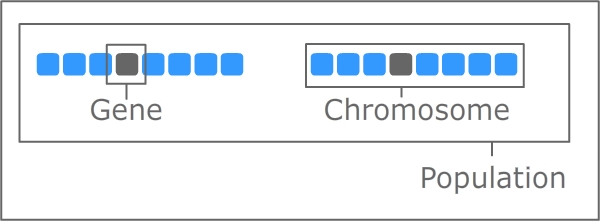
\includegraphics[scale=1.0]{gene_chromosomes.jpg}
\caption{gene, chromosomes and population description}
\label{fig:gene}
\end{figure}

\item \textbf{Initialisation of the population}
\item \textbf{evaluation function(fitness)}
\item \textbf{Genetic operators altering chromosomes(reproduction/selection, crossover and mutation.}
\item \textbf{Parameters for population size and probabilities of genetic operators.}
\end{itemize}



\subsubsection{Genetic Operators}
Genetic operators in some of the more simple Genetic Algorithms are reproduction/selection, crossover and mutation as described by Baltzer, 2014 and is elaborated by Melanie, 1990. \cite{Melanie1990}

\textbf{reproduction/selection:} \enquote{This operator selects chromosomes in the population for reproduction. The fitter the chromosome, the more times it is likely to be selected to reproduce.} \cite[pp. 8]{Melanie1990}
The idea behind this operator is that preferences are given to the better chromosomes in the population, which is then passed on to the next generation. This is based upon the fitness score.


\textbf{Crossover:} \enquote{This operator randomly chooses a locus and exchange the subsequences before and after that locus between two chromosomes to create two offspring.} \cite[pp. 8]{Melanie1990}


\textbf{Mutation:} \enquote{This operator randomly flips some of the bits in a chromosome.} \cite[pp. 8]{Melanie1990}




\subsubsection{GA and Pacman(how the two can be combined.(methods)}
we must identify possible implementations of "pacman parameters" to control fitness score.
